\chapter{Alternative modeling techniques}

This chapter deals with other possibilities of modeling the technical
system, particularly the double-acting pneumatic piston. Physical modeling
and data-driven modeling methods were examined in terms of suitability for
applying FDI and PdM strategies.

\section{Physical Modeling}
Physical modeling operates with models with a compiled layout that matches
the structure of the different physical domains. In this type of software,
it is possible to combine different domains to create a complex system
model.

Matlab/Simulink provides a physical modeling library, Simscape, that meets
the above specifications. Using Simscape software, the user combines a
model from different blocks representing different physical functions
(spring, resistance, hydraulic valve), and connection links represent some
types of energy flow.



\subsection{The double-acting pneumatic piston in Simscape}

In this part, the same assumption applies as in section \ref{assumptions}. All the
processes take place adiabatically, i.e., without heat exchange with the
environment. 

The resulting model was compiled using gas and mechanical domains \ref{simscape}.

\begin{figure}[h!]
    \centering
    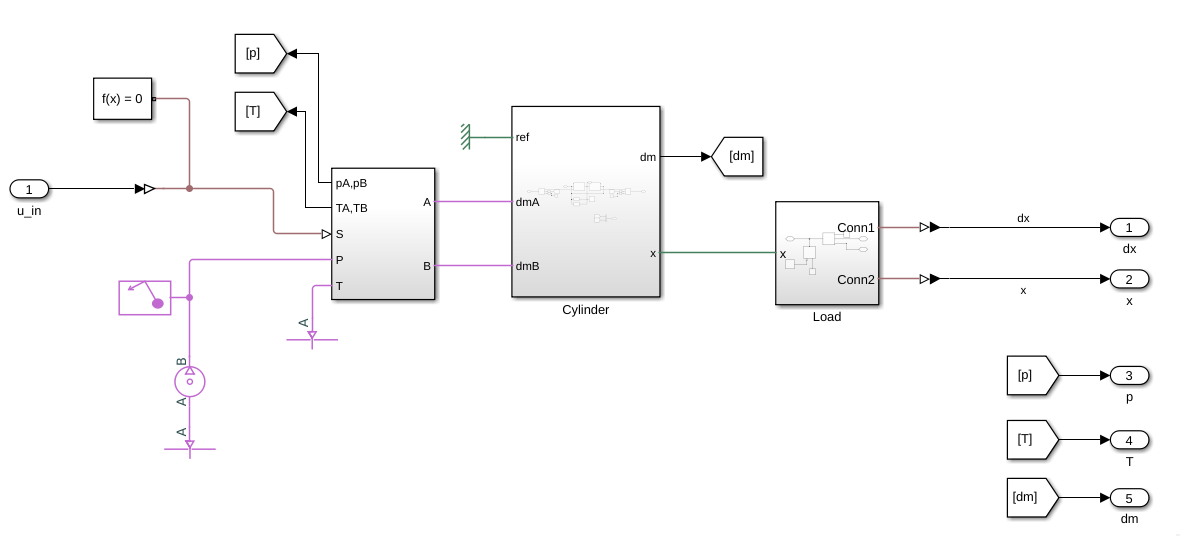
\includegraphics[width=1\textwidth]{simscape.png}
    \caption{The double-acting pneumatic piston developed using Simscape
    software}
    \label{fig:simscape}
\end{figure}


\subsection{Limitations}

It is necessary to know well the parameters of the system.

For example, we need to have a precision-measured characteristic of flow
control valve adjustment in the form of a lookup table to use a throttle
valve block.

Providing simplification and reduce the model to the only control valve,
there are still a few parameters that are not available such as valve and
dampers coefficients mentioned before \ref{}.

The main problem is the computational complexity of the model compared with
the first principle model. During the parameter estimation, the first
principle model is much faster than the Simscape model and gives an option
to experiment with different fault states analysis. 

However, both models showed quite close behavior during testing with the
same parameters; results shown in figure \ref{}.


\section{Data-Driven Models}

Between data-driven modeling techniques include:
\begin{itemize}
    \item Parametric
    \item Non-parametric
\end{itemize}

Non Parametric models include artificial neural networks and others.
